\chapter{データベースの基礎知識}\label{chap:concept-of-database}
今日，データベースは様々な業務やアプリケーションで利用されています．
例えば，Amazon\footnote{Amazon．\url{https://www.amazon.co.jp/}}や楽天市場\footnote{楽天市場．\url{https://www.rakuten.co.jp/}}といったオンラインショッピングサイトにおいては，購買履歴管理や在庫管理を行うためにデータベースが用いられています．
Instagram\footnote{Instagram．\url{https://www.instagram.com/}}やTiktok\footnote{Tiktok．\url{https://www.tiktok.com/}}といった，多数のユーザがコンテンツを投稿・閲覧するソーシャルメディアにおいてもデータベースは欠かせません．
個人用ブログのような比較的小規模なウェブサイトでも，記事データを管理するためにデータベースが用いられています（例: WordPress\footnote{WordPress．\url{https://ja.wordpress.org/}}．
このように，データを語る上でデータベースはなくてはならないものです．

本章では，データベースの概念を説明した後，最も代表的なデータベースであり，かつ本書の主要テーマでもある\strong{関係データベース}の概要について述べます．


% ---------------------------------------
\section{データベースとは}
% ---------------------------------------
データを収集・利用する文化が根付いてきたこともあり，データベースという言葉が市民権を得つつあります．
しかし，「データベース」という語が指す意味は，一般人とITの専門家とは大きく異なります．
第1章でも述べたように，一般の方にとってのデータベースとは「データの集まり」くらいの意味で捉えられていることが多いです\footnote{データと情報も明確に区別されることなく使われることが多いですが，情報学の世界では区別されています．データは「様々な活動や営為の結果得られる記号の集まり」であり，情報は「データが解釈され，意味や価値が付加されたもの」を指します．}．
一方，ITの専門家にとってのデータベースは，
\begin{quote}
``複数の応用目的での共有を意図して，組織的にかつ永続的に格納されたデータ群（北川博之著「データベースシステム」\cite{北川本}より）''
\end{quote}
あるいは
\begin{quote}
``データの正しさを管理する主体によって体系的に整理され，計算機によって永続的に格納されたデータの集まり（吉川正俊著「データベースの基礎」\cite{吉川本}より）''
\end{quote}
を意味します．
「データの正しさを組織的に管理する」という考えが強調されています．

データベースを扱うためのシステムは，\strong{データベース管理システム（database management system, DBMS）}と呼ばれます．
我が国のデータベース研究の大家である増永良文氏はその著者の中で，データベースとDBMSの関係を「料理」と「それを盛る器（うつわ）」の関係に例えています\cite{増永本}．
\begin{itemize}
\item データの正しさを組織的に管理するための「器」がDBMS
\item DBMSという器に盛られた「料理」，すなわち正しく管理されたデータの集まりがデータベース
\end{itemize}
という対応関係になります．
本来データベースとはDBMSによって管理されるデータ群を指しますが，データ管理の現場では，DBMSそのもの（あるいはDBMSとそれによって管理されるデータ群）をデータベース（DB）と呼ぶこともあります．

増え続ける多様かつ大量のデータと付き合っていくためには，データの\.う\.ま\.い管理・処理方法が必要になります．
場当たり的にデータを作ってはファイルとしてフォルダ（ディレクトリ）に突っ込んでおいたり，Excelシートにまとめていくというやり方は，扱うデータが増え，データを使う人間やアプリケーションが増えるにつれて，やがて破綻します．
ITの専門家が考えるデータベースは，こういった事態を未然に防ぐための強力なツールとなります．


% ---------------------------------------
\section{大規模なデータを扱う上での課題}
% ---------------------------------------
第1章の山畑さんの事例で見たように，大量のデータを適切かつ効率的に管理・処理するには，以下のような要件が求められます．

\subsubsection{多様かつ大規模なデータの管理}
ビジネスをはじめとする現場では，多種多様かつ大量のデータが時々刻々と発生しています．
例えば，2020年1月1日から2020年12月31日までの12か月間に，Amazon.co.jpで購買された商品の数は5億点以上にのぼるとされています\cite{DataVolumeOfAmazon}．

個人で管理する家計簿のような小規模な表データであれば，Excelのような表計算ソフトでも対応できます．
しかし，データの規模が大きくなり，様々な種類のデータが登録されるようになり，表データの登録・更新に関わる人が増えていくと…
やがてデータの管理が破綻するのは想像に難くありません．
何がどこに登録されているのかもよく分からなくなりますから，目当てのデータを探すのも大変です．
データの登録，修正，削除などなど，何をするのも大変になります．

そもそもExcelは1つの表につき最大100万行程度しか扱えません．
Excelのようなスプレッドシートでは，購買データのように数千万行，数億行もある多様かつ大規模なデータを効率よく蓄積，管理することは困難極まりないのです．


\subsubsection{データの正しさの保証}
管理するデータが大量かつ多様になってくると，データを正しく保つことが難しくなってきます．
特に，大量のデータを複数人，複数のグループや部署で扱うようになると，データの入力ミス，データ入力規則の無視，データ間の矛盾が発生しやすくなります．

当然ですが，管理対象となるデータに誤りが混入すると，そのデータを使うときに大変なことになります．
例えば，図\ref{fig:bad-data}のように，購買データの中に
\begin{itemize}
\item 現実にはあり得ない売り上げ金額が記録されている（データの入力ミス）
\item 入力形式が異なる日付が混在している（データの入力規則の無視）
\item 取扱商品リストにないはずの商品が購買履歴に含まれている（データ間の矛盾）
\end{itemize}
といったことが起きると，オンラインショッピング事業においては一大事です．
このような正しくないデータは直接参照されたときも問題になりますが，複数のデータを集計する際にも悪影響を及ぼします．
それゆえ，データ管理においては，格納されるデータの正しさ，データ間の矛盾のなさを保証する機能が求められます．

\begin{figure}[h]
    \centering
    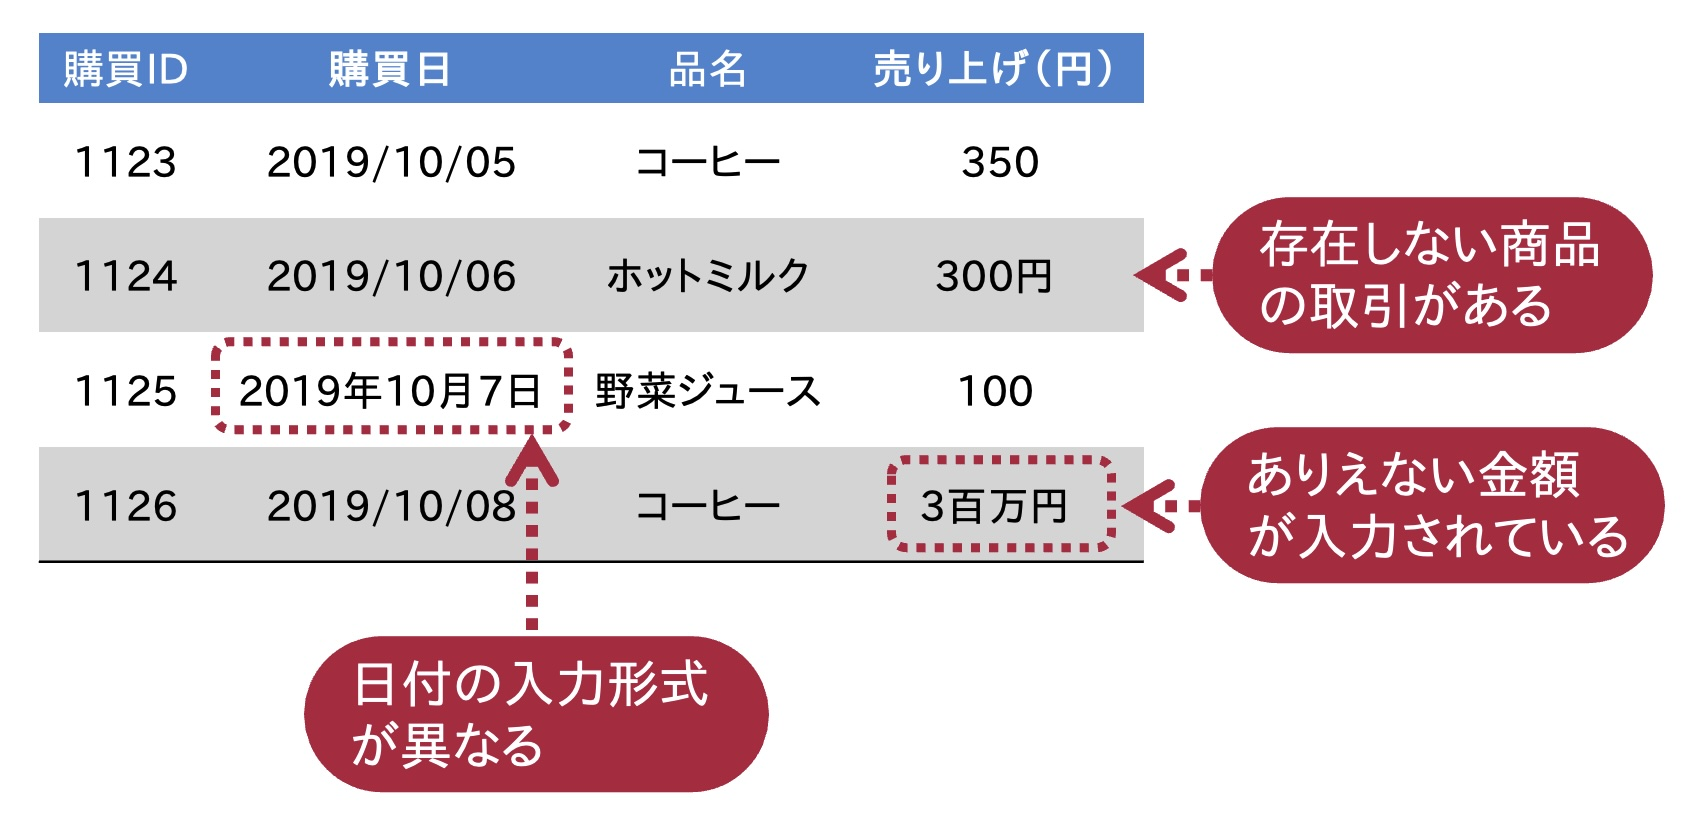
\includegraphics[width=1.0\textwidth]{figure/concept-of-database/bad-data.jpg}
    \caption{正しくないデータの例．}
    \label{fig:bad-data}
\end{figure}


\subsubsection{高速で効率的なデータ処理}
大量のデータを正しく管理できたとしても，対象となるデータを高速に処理できなければ実用的ではありません．
例えば，図書館における書籍の検索システムを考えてみよう．
たとえ数百万件の書籍情報を正しく管理する蔵書管理システムがあっても，ニーズにマッチする書籍のリストの検索に数分待たされるようでは，誰も使いたくありません．

一般に，あるシステムを利用するユーザが増えるにつれて，システムにかかる負荷も増えていきます．
例えば，Amazon.co.jpでは毎分平均900件以上の商品取引が行われています\cite{TransactionInAmazon}．
それゆえ，大量のデータが格納されているシステムにおいては，多発的に大量のデータのやりとりが発生することも想定して，高速かつ効率的なデータ処理が求められます（図\ref{fig:linear-search-for-table}）．

\begin{figure}[h]
    \centering
    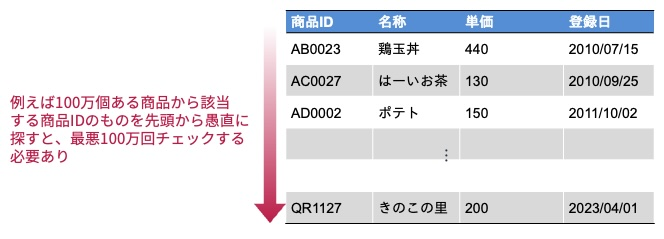
\includegraphics[width=1.0\textwidth]{figure/concept-of-database/linear-search-for-table.jpg}
    \caption{上から下に順に調べ上げていく線形探索では．大規模データに対する高速なアクセスは難しい．}
    \label{fig:linear-search-for-table}
\end{figure}


\subsubsection{同時実行（並列処理）}
関連して，大勢の人が同時にデータを追加，更新，削除しても，管理中のデータに矛盾が生じないようにシステムが動作することも重要です．

例えば，Xさん，Aさん，BさんがPoyPoyという名称のコード決済システムを利用しているとしましょう．
最近のコード決済システムはお店にお金を支払うだけでなく，ユーザ同士でお金を送金しあうこともできます．
さて，XさんのPoyPoy口座残高は5万円とします．
一般に，口座への送金があった際，送金先口座の残高の計算は
\begin{quotation}
残高 = 送金時の「送金先口座」の残高 + 送金額
\end{quotation}
送金元口座の残高の計算は
\begin{quotation}
残高 = 送金時の「送金元口座」の残高 - 送金額
\end{quotation}
となります．
これは至極当然の処理ですが，次のような状況を考えてみましょう．

ある日，Xさん，Aさん，Bさんは食事に出かけ，XさんがAさん，Bさんの代金を立て替えたとします．
AさんとBさんは，PoyPoyアプリを通じてXさんに立て替えてもらった金額（3000円）を精算することにしました．
さて，AさんとBさんは，XさんのPoyPoy口座に\strong{まったく同じタイミングで}3000円送金したとします．
この際，前述の計算式をそのまま適用すると，図\ref{fig:mutual-exclusion}のように誤った処理が行われてしまいます．
\begin{figure}[tb]
    \centering
    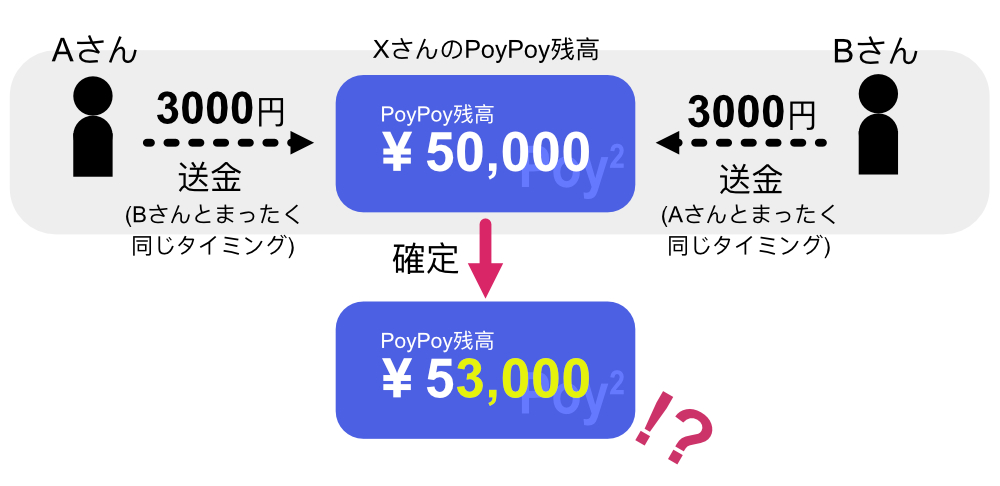
\includegraphics[width=0.8\textwidth]{figure/concept-of-database/mutual-exclusion.jpg}
    \caption{複数の処理要求を矛盾なく処理できていない例．}
    \label{fig:mutual-exclusion}
\end{figure}
AさんとBさんが送金を行った後，Xさんの口座の残高は5万3000円になりました -- こんなことが起きたら大変ですよね．
この例における問題点は，たとえ振込み処理が同時に発生したとしても，Aさんの振り込み処理を待ってからBさんの処理を行うべきであったという点です．

このように，データ処理の内容によっては，別の処理が完了したことを保証してから次の処理を行う必要があります．
さらに，処理の途中で何らかのエラーが起きた場合は，すべての処理をキャンセルして最初の状態に戻すことが求められます．
データを管理しているシステムに同時アクセスがあった場合でも，データを矛盾なく処理できることが重要となります．


\subsubsection{アクセス権限のコントロール}
データによっては，誰でも自由に閲覧してよいものもあれば，特定の立場のユーザしかアクセスできないようにすべきものも存在します．
多種多様なデータのやりとりが発生する環境においては，ユーザの属性ごとにデータの閲覧，作成，更新，削除といったアクセス権限を制御する機能が必要となります．


% ---------------------------------------
\section{データベースを用いるメリット}
% ---------------------------------------
一人で扱えるほどデータの規模が小さければ，Excelなどの表計算用のソフトウェアでデータ管理しても問題はありません．
しかし，扱うデータが多様かつ大規模になると，問題が生じなくするために要求されるデータ処理の質が変わります．
そのため，データの管理方法や処理方法を見直す必要があります．

本稿で学ぶデータベースを用いれば，\strong{データの一元管理}が可能となり，データの管理や利活用において様々な恩恵を受けられます．
具体的には，データベースが備える以下のような特性あるいは関連技術を用いることで，前節で述べた「大規模なデータを扱う上での課題」をクリアすることができます．
\begin{itemize}
\item 大規模なデータの管理：「\strong{物理的データ格納方式}」の工夫によって対応
\item データの正しさの保証：「\strong{一貫性制約}」によって対応
\item 高速で効率的なデータ処理：「\strong{索引づけ}」「\strong{問い合わせ最適化}」などで対応
\item 同時実行，データの共同利用：「\strong{トランザクション}」などで対応
\item アクセス権のコントロール：「\strong{ロール管理}」によって対応
\end{itemize}



% ---------------------------------------
\section{関係データベース超入門}
% ---------------------------------------
これから本書で学ぶ\strong{関係データベース（relational database）}とは，あらゆるデータを\strong{表（table）}\footnote{表のことをテーブルと呼ぶこともある．}の形式で管理するデータベースです\cite{Codd1970}．
第3章で述べるように，実はデータベースといっても様々な種類のものがありますが，関係データベースはその中でも最も代表的なものです．
関係データベースを管理するためのシステム（すなわちDBMS）は，\strong{関係データベース管理システム（relational database management system，略してRDBMS）}と呼ばれています．

\begin{figure}[h]
    \centering
    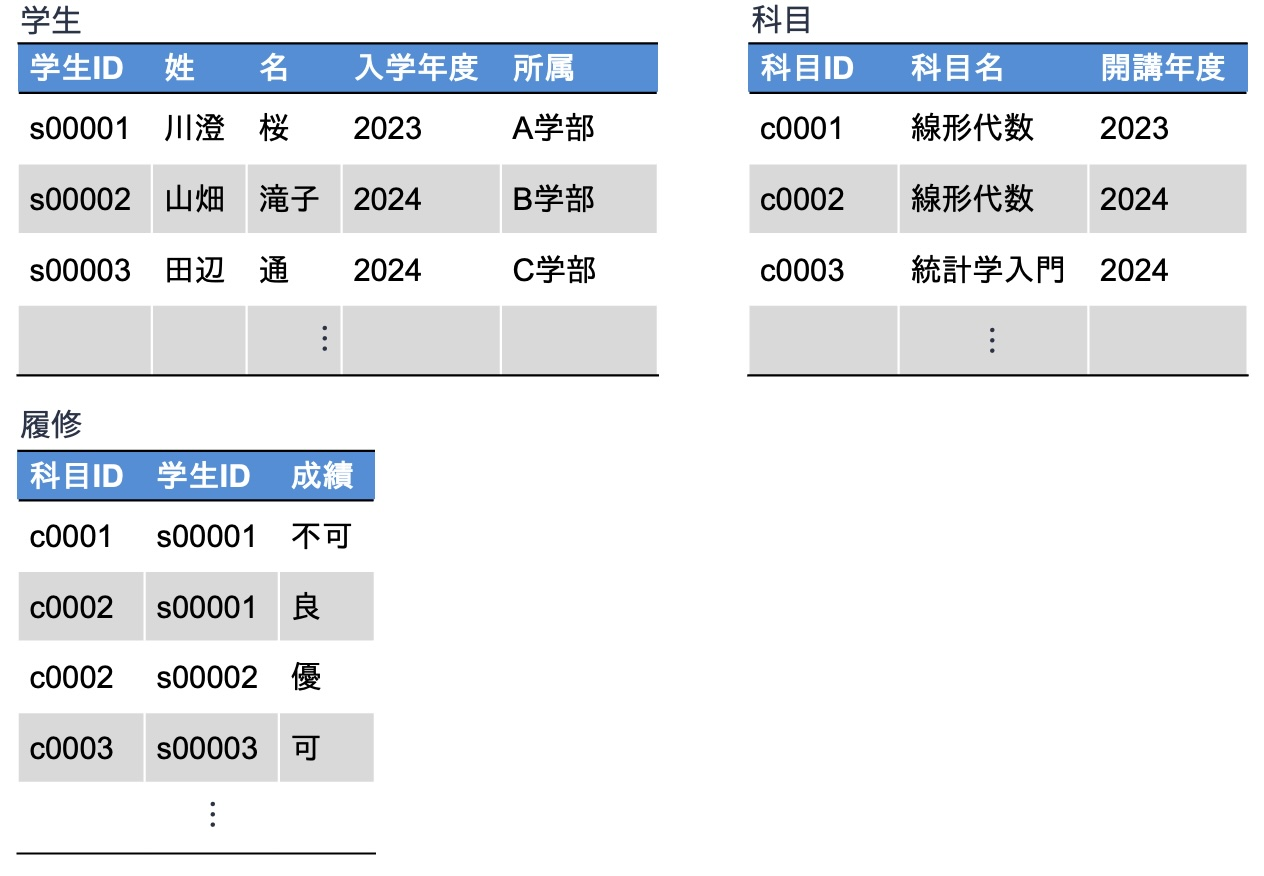
\includegraphics[width=1.0\textwidth]{figure/concept-of-database/example-of-relation.jpg}
    \caption{関係データベースの例．}
    \label{fig:example-of-relation}
\end{figure}

図\ref{fig:example-of-relation}は，授業の履修状況・成績を管理する関係データベースの例です．
この関係データベースには，以下の3つの表が存在しています．
\begin{itemize}
\item 学生テーブル：学籍番号，氏名，入学年度，所属といった学生に関する情報を格納
\item 科目テーブル：科目ID，科目名，開講年度といった科目に関する情報を格納
\item 履修テーブル：どの学生が何の科目を履修し，どのような成績であったかに関する情報を格納
\end{itemize}
各表は行と列から構成されており，各行には表が扱うデータが格納されています．
図\ref{fig:example-of-relation}の学生テーブルを例に取ると，各行のデータは学生一人一人の情報を表しています．
関係データベースでは，行のことを\strong{タプル（tuple）}あるいは\strong{レコード（record）}と呼びます．
各レコードは，表の見出しに対応するデータの値を持ちます．
各見出しのことを\strong{属性（attribute）}，属性に対応するレコードの値を\strong{属性値（attribute value）}と呼びます．
学生テーブルの例では，学生ID，姓，名，入学年度，所属が属性に対応し，一番上に書かれているレコードの属性「学生ID」の属性値は\graybox{s00001}となっています．

この例だけ見ると「なんだ，関係データベースは単なる表じゃないか」と思われたかもしれませんが，\strong{ただの表ではありません}．
一見するとただの表にしか見えませんが，データを正しくかつ効率よく管理・処理するために，あらかじめ定義された「データの構造」「データの制約」「データの操作」に関する規則に従ってデータが作られ，関係データベース内に格納されます\footnote{データの構造，制約，操作に関する規則を定めたものを「データモデル」と呼びます．データモデルについては，第3章で詳しく述べます．}．
例えば図\ref{fig:example-of-relation}の関係データベースであれば，以下のような規則に従い，授業の履修状況や成績を管理するための情報が複数のテーブルに分割され，データベース内に格納されています：
\begin{itemize}
\item 学生テーブルは「学生ID」「姓」「名」「入学年度」「所属」という属性をもつ
\item 学生テーブルの「学生ID」や科目テーブルの「科目ID」はテーブル内で値が重複することはない
\item 履修テーブルには，科目名や学生の氏名といった科目や学生の詳細情報は格納しない
\item 履修テーブルの成績には「優」「良」「可」「不可」のいずれかしか登録できない
\item 履修テーブルに現れる科目IDおよび学生IDは，必ず学生テーブルと科目テーブルに存在する
\end{itemize}

少し詳しく見てみましょう．
図\ref{fig:primary-key}のように，学生テーブルの「学生ID」は重複することがないため，その値が決まれば学生の情報が一意に決まります（どの学生かが特定できる）．
このような属性（またはその組み合わせ）テーバーン委データベースでは\strong{主キー（primary key）}と呼びます．

\begin{figure}[h]
    \centering
    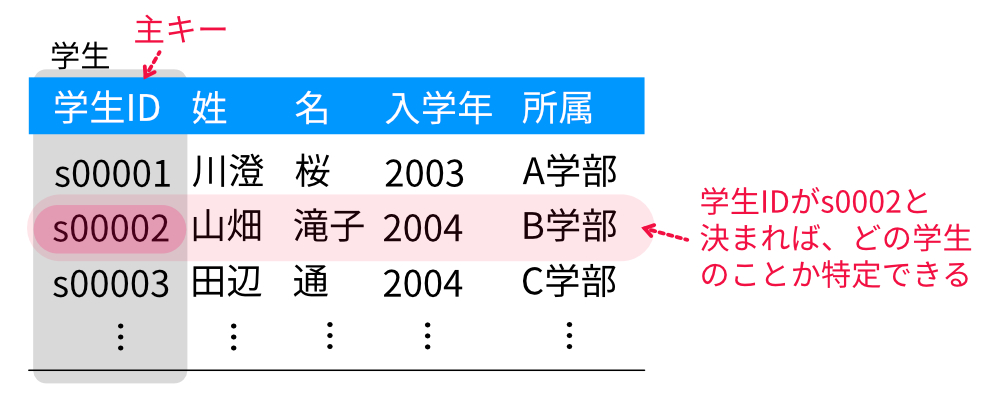
\includegraphics[width=0.8\textwidth]{figure/concept-of-database/primary-key.jpg}
    \caption{主キーの役割}
    \label{fig:primary-key}
\end{figure}

履修テーブルはどの学生が何の科目を履修し，どのような成績であったかを管理するための表ですが，学生の具体的な情報は保持せず，学生IDのみを保持しています．
学生の姓や名，所属といった情報が欲しい場合は，学生IDを手がかりに学生テーブルを参照すれば取得できます．
同じことは科目情報についても言えます．
これは見方を変えると，履修テーブルに格納された学生IDや科目IDは，必ず学生や科目の詳細情報を参照できるよう，必ず学生テーブルや科目テーブル内に存在している必要がある，ということになります．
このように，他のテーブルでは主キーとなっていて，それを手がかりにすることで関連情報を参照するための属性を，関係データベースでは\strong{外部キー（foreign key）}と呼びます．
図\ref{fig:foreign-key}の例では，履修テーブルにおける学生IDや科目IDは（学生テーブルや科目テーブルに対する）外部キーとなっています．
（直感的なイメージとしては）外部キーは，ウェブページにおけるハイパーリンクのような役割を果たしています．
先の例で言えば，履修テーブルの学生IDをクリックすると，学生テーブルから該当学生の詳しい情報が見れる，といったイメージです．
このような仕組みによって，関係データベースは情報が冗長にならないように整理整頓されています．

\begin{figure}[h]
    \centering
    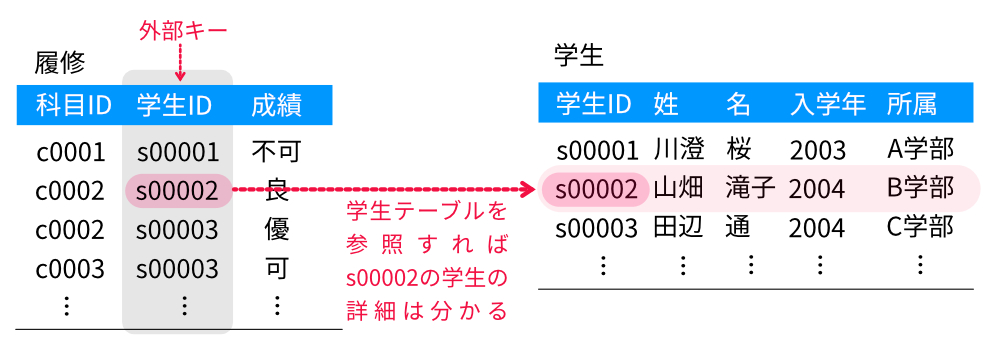
\includegraphics[width=1.0\textwidth]{figure/concept-of-database/foreign-key.jpg}
    \caption{外部キーの役割}
    \label{fig:foreign-key}
\end{figure}

なぜ履修テーブルに学生や科目の詳細情報も載せないのでしょうか．
それは，学生や科目の詳細情報が変更された場合に，履修テーブル内の情報もすべて更新しなければならなくなるからです．
もしすべての情報を1つの表にまとめていたら，どうなるでしょうか．
例えば，山畑さんが在学中にB学部からD学部に転部し，所属が変わったとしましょう．
この場合，もし履修テーブルに山畑さんに関する情報が100件登録されていたら，100件すべての所属をB学部からD学部に書き換えなければなりません．
その際，もし1件でも書き換え忘れがあったら，B学部の山畑さんとD学部の山畑さんが混在することになり，正しい成績証明書が出せなくなってしまいます．
図のように，学生や科目の詳細情報を履修テーブルとは別のテーブルに分けておけば，学生や科目の詳細情報が変更された場合でも，学生テーブルや科目テーブル内の情報を1か所更新すれば済みます．
このような工夫も，関係データベースの重要な特徴の1つです．

上記のような工夫はデータの正しさを保証するためのものでしたが，他にも関係データベースにはデータの検索・集約を効率よく行うための仕組みや同時アクセスの制御など，データを適切に扱うための様々な仕組みが備えられています．
次章以降では，
\begin{itemize}
\item 一見ただの表にしか見えない関係データベースが，どのような理論に基づいて定式化されているか
\item 関係データベースをどのように設計するのか
\item 関係データベースを用いると，なぜ大規模データの管理が効率的になるのか
\end{itemize}
などについて詳しく述べていきます．


% ---------------------------------------
\hrulefill
\section{クイズ}
% ---------------------------------------
\subsubsection{Q1. メジャーなデータベース管理システム}
ウェブ検索エンジンを用いて，世の中にあるメジャーなデータベース管理システムを調べなさい．
また，調べたデータベース管理システムを「関係データベースを扱うもの」と「そうでないもの」に分類しなさい．

\subsubsection{Q2. 線形探索}
100万件ある商品リストの中に特定の商品が含まれているかを確認したいとします．
商品リストの先頭から末尾まで順に商品名を確認していくと，平均で何回（何件）の確認で商品の有無を確認できるでしょうか．

\subsubsection{Q3. データベース管理システムの利用例}
普段利用しているサービスのうち，データベース管理システムを用いていると思われるものを3つピックアップしなさい．

\subsubsection{Q4. CSV/TSVファイル}
CSVファイルおよびTSVファイルとは何かを調べなさい．
また，（データベース管理システムでデータを管理する場合と比較して）CSV/TSVファイルに存在する欠点を挙げなさい．

\subsubsection{Q5. チューリング賞}
関係データベースの理論的基盤である関係モデルを提唱したEdgar F. Codd氏は，計算機科学分野のノーベル賞といわれるチューリング賞の受賞者である．
Codd氏以外で，データベースに関する功績でチューリング賞を受賞した人をピックアップしなさい．
